\documentclass[12pt,oneside,reqno]{amsart}
\usepackage[left=3cm,right=3cm,top=5cm,bottom=2cm]{geometry} % page settings
\usepackage{amsmath} % provides many mathematical environments & tools
\usepackage{amssymb}
\usepackage{tikz}
\usepackage{graphicx}
\usepackage{hyperref}

\begin{document}
\setlength{\parindent}{6pt}
\def\code#1{\texttt{#1}} %Code looking
\DeclareGraphicsExtensions{.pdf,.png,.jpg}

\title{TIN093 Exercise week 5}
\author{Josefin Ondrus}
\date{\today}
\maketitle

%***********OK**************A
\textbf{A. Let $n$ and $m$ denote the number of nodes...}\\\\
%*************************
Given: $n,m$ - the number of nodes and edges in a connected graph.\\
Could $O(m)$ and $O(n+m)$ represent the time bound for the same algorithm?\\\\
I'll argument that they can. If we only look at the numbers and what type of graph it is (which we have to, since we have no further info about the algorithm), we could make some statements regarding the relationship between $n$ and $m$.\\\\
In a connected graph, the smallest number of edges possible is $n-1$.\\
Assuming the graph is undirected, the maximum number of edges possible is $\frac{n(n-1)}{2}$\\
Assuming the graph is directed, the maximum number of edges possible is $n(n-1)$.\\
(However, it will not matter whether the graph is directed or undirected so we assume it is undirected for now.)\\\\
According to the statements above. We know that $n-1 \leq m \leq \frac{n(n-1)}{2}$. This means that the only time $m$ could be bigger than $n$ is when $m$ is as small as possible. If we would compare the two time bounds in both cases we'll get the following differences:\\\\
For the smallest $m$:\\
$O(m)=O(n-1)$\\
$O(n+m)=O(n+(n-1))=O(2n-1)$\\
Taking only the dominating factor in consideration, we see that they are equal.\\\\
For the largest $m$:\\
$O(m)=O(\frac{n(n-1)}{2})=O(\frac{1}{2}(n^2-n))$\\
$O(n+m)=O(n+\frac{n(n-1)}{2})=O(\frac{1}{2}(2n+n^2-n))=O(\frac{1}{2}(2n^2+n))$\\ 
As with the smallest $m$ the dominating factor in both cases are equal. (If it would've been a directed graph, it would result in $O(2n^2+n)$), making no difference to th dominating factor.)\\\\
Hence we can argue that both time bounds can represent the same algorithm and none of them have to be mistaken. It is most likely a difference in how strict they've calculated the bounds. 


%***********OK**************B
\textbf{B. Why can we write $O(m log n)$ instead of...}\\\\
%*************************
As mentioned above, we can describe $m$ within an interval depending on $n$ as: $n-1 \leq m \leq \frac{n(n-1)}{2}$. If we would compare the two different expressions we can come to the following conclusions:\\\\
$O(mlog(n-1))$ is such a small difference from $O(mlogn)$ and they both have the same growth as $m,n$ increases.\\\\
$O(mlog(\frac{n(n-1)}{2}))=O(m(log(n(n-1))-log2))=O(m(logn+log(n-1)-log2))$, if we ignore the slower growing factors we get a time bound of $O(mlogn)$. \\\\
If it would have been a directed graph, the difference in the max number of edges would only affect the slower growing factors, resulting in the same result as for the undirected graph.\\\\

%************************C
\textbf{C. Suppose that we have executed depth-first search...}\\\\
%*************************
"Every cycle in the graph only consists of tree edges and one back edge." is ture.\\\\
Let's start with the definition of a back edge - "If in edge $(u,v)$, $v$ is the discovered already and $v$ is an ancestor, then $(u,v)$ is a back edge." This would clearly be the case in every cycle, since we always need to "close the cycle" for it to be a cycle and since we have an undirected graph, we cannot get cross-edges nor forward-edges in our DFS tree, hence, the cycle can only consist of tree edges and one back edge.\\\\
The algorithm I propose is a DFS where we for every time we check a node and it is marked as visited, we check that it's not the parent node of our current node in the BFS tree. If not, we return true since the graph then have a cycle. Since the time for a DFS is $O(m+n)$ and our extra check gives us a constant addition to the time complexity, we can ignore this and this gives our algorithm a time bound of$O(m+n)$.\\\\
\newpage
%*************************D
\textbf{D. Can an articulation point belong to...}\\\\
%*************************
Yes! See below example where node 4 is an articulation point and a part of the circle $4->5->2->3->4$.\\\\
\begin{tikzpicture}
  [scale=.5,auto=right,every node/.style={circle,fill=white!20}]
  \node (n1) at (1,6) {1};
  \node (n6) at (1,10) {6};
  \node (n4) at (4,8)  {4};
  \node (n5) at (8,9)  {5};
  \node (n2) at (9,6)  {2};
  \node (n3) at (5,5)  {3};

  \foreach \from/\to in {n6/n4,n4/n5,n6/n1,n2/n5,n2/n3,n3/n4}
    \draw (\from) -- (\to);

\end{tikzpicture}\\\\
%*************************E
\textbf{E. We have seen how BFS can be used to test...}\\\\
%*************************
Suppose we are traversing a graph using DFS. While traversing, we not only construct the DFS tree but we also check for back-edges. If we find a back-edge we check the difference between the DFS-tree levels of the current node and the node where the back-edge ends. If the difference between the current node and the end-node is an even number, we know that the graph is not bipartite. (Would it be better to explain by pseudo code? For the exam, I mean...)\\\\

Since a bipartite graph is a graph that does not contain any odd-length cycles we can determine weather the graph is bipartite by checking the cycles. We know (from previous question C.) that every cycle in a graph only consists of tree edges and one back-edge. This means that we discover every cycle when we discover a back-edge. Now, the only thing that remains to check is weather the cycle is of even or odd length. This we can do by counting the nodes that are a part of the cycle. This we can do by comparing the levels of the both nodes involved in the back-edge. If the difference between between the levels is an even number, we know that the number of nodes involved in the cycle is an odd number of nodes. (The difference gives us the number of edges involved in the cycle before the back-edge is added. Adding the back-edge results in an cycle of an odd number of edges, resulting in an odd number of nodes.)\\\\
\newpage
%*************************F
\textbf{F. We run Kruskal’s algorithm to get a clustering...}\\\\
%*************************
“The length of any selected edge inside a cluster is smaller than the spacing.”\\
This statement is true. Since we're using Kruskal's algorithm which inserts an edge between nodes in increasing order, we know that the edge of greatest distance will be saved for last and hence we know that the length of any selected edge inside a cluster is smaller than the spacing.\\\\
 – “The distance between any two nodes inside a cluster is smaller than the spacing.”\\
 This statement is false. The information is in the edges "produced" by Kruskal's algorithm, hence we don't know the length information if two nodes are not connected. Just that there is a smaller edge that can connect one node with the rest of the cluster if no edge exist between two nodes in the same cluster. See graph below for counterexample.\\\\
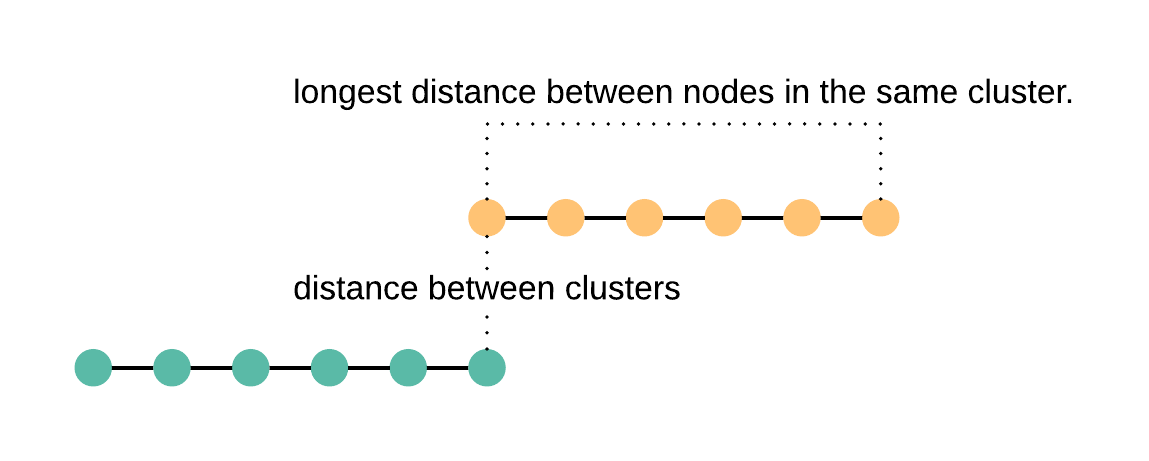
\includegraphics[scale=1.5]{cluster.png}\\
%*************************EXAM
\textbf{Can be exam-related. Suppose that a cleaning robot can walk...}\\\\
%*************************
Suppose the number of edges is $m$ and the robot have to go through every corridor the robot will have to do at least $m$ edge traversals. But we also need to get back from every crossing (including the leafs) and the robot can only do this by going back the same way he came from since a tree can't have any cycles. If we program the robot with the DFS algorithm we can clean all the corridors and get back in $2m$ edge traversals. Which also is the smallest number of traversals possible if it is a tree structure because of the absence of cycles.
\begin{figure}[b]
    \href{https://www.youtube.com/watch?v=tLt5rBfNucc}
         {
\includegraphics[scale=0.5]{robot}}
\end{figure}\\

\end{document}